\documentclass[11pt]{article}

\usepackage[ruled,vlined,linesnumbered]{algorithm2e}

\usepackage{times}
\usepackage{anysize}
\usepackage{graphicx}
\usepackage[ruled,vlined,linesnumbered]{algorithm2e}


\marginsize{2cm}{2cm}{2cm}{3cm}
%\onehalfspace
%\doublespace
\setlength{\parindent}{0.8cm}
%\setlength{\parskip}{0.2\baselineskip}
%\setlength{\topmargin}{2cm}
%\setlength{\textheight}{25cm}
%\setlength{\textwidth}{14cm}
%\setlength{\oddsidemargin}{2cm}
%\setlength{\evensidemargin}{2cm}
\usepackage{fancyhdr}
\pagestyle{fancy}

\newcommand{\note}[1]{\textbf{\textit{#1}}}
\newcommand{\vac}[2]{\textit{Vacuumed(#1,#2)}}
\newcommand{\move}[3]{\textit{Move$_{#1}$(#2,#3)}}
%\newcommand{\move}[3]{\textit{Move(#1) BLA #2,#3}}
\newcommand{\at}[3]{\textit{At$_{#1}$(#2,#3)}}

%\newcommand{\vac}[2]{\textit{Vacuumed(t=#1,#2)}}
\newcommand{\astar}{A$^*$}

\newtheorem{theorem}{Theorem}
\newtheorem{observation}{Observation}
\newtheorem{corollary}{Corollary}

\linespread{1.3}

\lhead{Interaction Oriented Multi-Agent Planning} \rhead{ISF 210/17 -- Roni Stern}
\cfoot{\thepage} 
%\cfoot{} 
\pagenumbering{arabic}
%\pagenumbering{Roman}




\begin{document}



\noindent {\LARGE Detailed Description of the Research Program}

\section{Scientific Background}
% From ISF guidelines: includes an overview of the research in the chosen topic

% Test


Data mules~\cite{shah2003data} is a low-cost technology for maintaining sparse connectivity. 




% The MAP problem and how much it is important and applied 
Imagine a smart home with a vacuum cleaning robot, a floor scrubbing robot, and a floor mopping robot (Figure~\ref{fig:example} illustrates this setting). This team of robots is committed to the overall mission of cleaning the house, with each robot having a specific task to perform: vacuum cleaning, floor scrubbing, or floor mopping. To accomplish their tasks, these robots must plan, either upfront or on-the-fly, the individual actions they intend to perform. In many cases, they must also coordinate these individual actions if they are to succeed in their overall mission. Similar issues arise in many other multi-agent systems (MAS), including automated warehouses~\cite{martinez2010autonomous,vivaldini2011intelligent} and teams of delivery robots~\cite{coltin2014scheduling}.  Analogous multi-agent planning (MAP) problems also arise in non-robotic scenarios, including teams of web crawlers~\cite{chiu2005towards,pant2002myspiders,sato2012agent} and digital entertainment~\cite{jaklin2013way}.  
%groups of AI characters in digital role-playing games~\cite{mott2006u,botea2013pathfinding,jaklin2013way}.  
%The importance of adequate MAP mechanisms for group activities is recognized in a range of formal models of teamwork~\cite{grant2005formalApproaches} and is becoming increasingly important with the greater prevalence of household and industrial robots as well as other types of multi-agent systems. 
The importance of adequate MAP mechanisms for group activities is recognized in formal models of teamwork and is becoming increasingly important with the greater prevalence of household and industrial robots as well as other types of MAS. %~\cite{grant2005formalApproaches}


%MAP algorithms are %, and in mixed networks of humans and machines~\cite{amir2013collaborative}.The entities that act in these scenarios (robots, crawlers, etc.) are generally called {\bf agents} and the task of planning for them is called {\bf multi-agent planning} (MAP). 


% The problem: MAP is much harder due to interactions. Existing planners can't scale because of this.





 % There are many MAP formalisms and algorithms. MAP is hard because need to reason about potential interactions
MAP has many variants and many formal models have been proposed to describe a broad range of MAP problems, including COM-MTDP~\cite{pynadath2002communicative}, Multi-Agent STRIPS (MA-STRIPS)~\cite{brafman2013complexity}, TAEMS~\cite{Horling-182,lesser2004evolution}, Decentralized POMDP (Dec-POMDP)~\cite{bernstein2002complexity}, and its variants~\cite{becker2004decentralized,roth2007exploiting,oliehoek2012influenceBased}. It is widely acknowledged across all MAP formalisms, that {\bf multi-agent planning is inherently more difficult than single-agent planning}, because agents need to reason not only about their individual plans but also about potential {\em interactions} between them, i.e., finding ways in which agents can help each other (positive interactions) and making sure that executing one plan does not prevent the execution of another (negative interactions).


% There are MAP algorithms, but they cannot scale because there are too many potential interactions
Many general-purpose MAP algorithms were previously proposed~\cite{torreno2014fmap,nair2005networked,witwicki2010influence,spaan2011scaling,oliehoek2012influenceBased,wu2013monte,dibangoye2014exploiting,nissim2014distributed}. We refer to these extant MAP algorithms as ``baseline planners". 
%~\cite{nair2003taming,nair2005networked,spaan2008interaction,oliehoek2008optimal,bernstein2009policy,witwicki2010influence,amato2010optimizing,spaan2011scaling,oliehoek2012influenceBased,wu2013monte,dibangoye2014exploiting,maliah2014privacyPreserving,maliah2015privacy,nissim2014distributed}. We refer to these extant MAP algorithms as ``baseline planners". 
Most baseline planners embody the assumption that the set of potential interactions that need to be considered during planning are specified in, or easily derived from, the problem description given to the planner. For example, in MA-STRIPS~\cite{brafman2013complexity} and in Nearly Decomposable MDP (NeDMDP)~\cite{kamar2013modeling} the agents' actions are partitioned into private/individual actions and public/joint actions, and potential interactions occur only when performing public/joint actions. In some Dec-POMDP variants, inter-agent influences are 
limited to the reward function (having the agents' transitions and observations independent of each other), or to predetermined situations~\cite{varakantham2009exploiting,melo2011decentralized}, or 
represented in a dynamic Bayesian network~\cite{nair2005networked,witwicki2010influence,oliehoek2012influenceBased}. 

\begin{figure}[h]
\centering
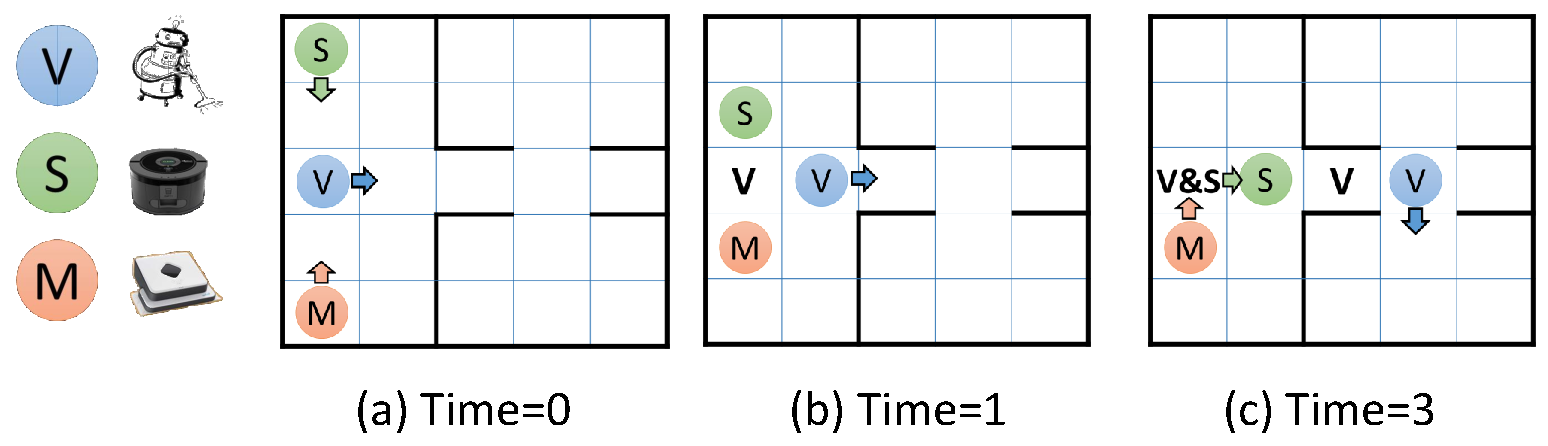
\includegraphics[width=0.7\columnwidth]{RunningExample_cropped.pdf}
\vspace{-0.4cm}
\caption{\small{An illustration of our smart home example. The vacuum cleaning robot, floor scrubbing robot, and floor mopping robot are marked by a circle with the letter V, S, and M, respectively. Collisions should be avoided and it is easier to scrub or mop the floor after it is vacuumed. Thus, to clean the house efficiently, a MAP algorithm is needed to coordinate the robots. The figure illustrates a start of a possible joint plan in which robot V starts immediately (at time=0) to vacuum the floor (vacuumed tiles are marked by V), while robot S decided not to scrub any floor that was not vacuumed, finishing to scrub his first floor tile time=3 (marked by adding the letter S on the tile). }}
\label{fig:example}
\end{figure}

{\bf Explicitly reasoning about all potential inter-agent interactions when planning severely limits the applicability of current MAP algorithms}, because the number of potential interactions can be large and MAP complexity is, roughly, exponential in the number of interactions reasoned about~\cite{brafman2013complexity,witwicki2011towards}. For example, in the above smart home scenario, each movement of one robot may interact with the movements of the other two robots, say, by possibly causing a collision. Thus, every move action of an individual robot raises a potential interaction (for example, in MA-STRIPS it would be a public action). % and most baseline planners will considered its interaction with the actions of all other robots when planning. % TODO: Reconsider the above sentence
Baseline planners would then reason about interactions with other robots for every movement of every robot. This is clearly not efficient and will not allow scaling to larger teams of robots. 
%Indeed, most baseline planners cannot scale beyond 10 agents. 
Indeed, most benchmark problems used to evaluate baseline planners rarely include more than 10 agents~\cite{vstolba2015competition}. 
%Reasoning about interactions with other robots for every movement of every robot is clearly not efficient and will not allow scaling to larger teams of robots. Indeed, most baseline planners cannot scale beyond 10 agents. 
The main goal of the proposed research is to develop a novel algorithmic framework, which we call {\bf interaction-oriented planning (IOP)}, that addresses the lack of scalability of current MAP algorithms by {\bf carefully considering which interactions should be reasoned about, how to reason about them, and when}. 


% Our IOP proposes: interactions is a complicated thing
In designing and developing the IOP framework, we will focus on the following key, fundamental capabilities: 
(1) algorithms for identifying and classifying potential inter-agent interactions that are relevant for planning,
(2) cost-aware coordination mechanisms for handling inter-agent interactions when planning,
(3) meta-reasoning algorithms for deciding rationally which potential inter-agent interactions can and should be ignored when planning and handled during execution, and (4) principled methods for deciding when a sufficiently coordinated and effective joint plan is found. 


\section{Research Objectives and Expected Significance}
Our overarching goal in this proposal is to deepen the understanding of MAP problems and develop a general-purpose algorithmic framework that will enable planning for larger and more diverse groups of agents. 
This goal will be addressed in the following four specific objectives, each of which has both fundamental theoretical and algorithmic challenges.

\subsection{Objective \#1: Algorithms for Identifying and Reasoning About Potential Interactions}

%\item {\bf Develop algorithms for identifying and reasoning about potential inter-agent interactions.} These algorithms will consider and exploit the difference between negative and positive interactions as well as the level of cooperation needed between the agents. 


%\subsubsection*{Generalizing Domain-Specific MAP}
While MAP is computationally hard and general-purpose planners do not scale~\cite{bernstein2002complexity,witwicki2011towards,brafman2013complexity}, there are specific MAP problems that can be solved efficiently even for a very large number of agents. One such MAP problem that spawned this research is the multi-agent pathfinding (MAPF) problem. MAPF can be solved suboptimally in polynomial time~\cite{wang2009tractable,de2013push,roger2012non} and recent optimal solvers, developed by the PI and others, can scale to more than a hundred agents~\cite{sharon2015conflict-based,sharon2013increasing,wagner2015subdimensional,boyarski2015don,boyarski2015icbs,barer2014suboptimal-socs,CohenUK15}, much more than the number of agents solved by current general-purpose MAP solvers~\cite{dibangoye2014exploiting,maliah2014privacyPreserving}. Another example of domain-specific MAP that scales to a large number of agents is multi-robot coverage, in which multiple robots need to cover an area together~\cite{agmon2008giving}. 
%In contrast, state-of-the-art general-purpose MAP solvers can rarely scale beyond ten agents~\cite{dibangoye2014exploiting,maliah2014privacyPreserving}. %IOP will be designed To develop IOP as a general algorithmic framework We will investigate the factors the differentiate 
Our hypothesis in developing IOP is that {\bf analyzing the form and degree of coordination needed for the agents to accomplish their mission will enable using techniques from domain-specific MAP algorithms} to handle potential inter-agent interactions and solve general MAP problems much more efficiently. % greatly improve the efficiency of solving general MAP problems.

\subsubsection{Analyzing Forms of Coordination}
%{\bf 1. Forms of coordination.} 
Although the specific ways in which agents' may coordinate vary widely, fundamentally each inter-agent interaction is either a positive or a negative one~\cite{cox2009efficient}. A negative interaction represents a case where agents' actions conflict in some way. For instance, the floor scrubbing agent may block the way of the vacuum cleaning robot. A positive interaction represents a case where one agent's actions assist another agent's task execution in some way. For example, the vacuum cleaning robot can make it easier for the floor scrubbing robot to do its work by vacuuming each tile before it is washed (as done in time steps 1 \& 3 in Figure~\ref{fig:example}). Ideally, MAP will avoid generating negative interactions and realize helpful positive interactions. 

We will explore suitable methods for identifying and handling both types of potential interactions and {\bf investigate ways in which the distinction between negative and positive interactions can be exploited in solving MAP problems}. For example, a MAP problem that does not allow for positive interactions is reducible to a MAPF problem, and therefore this MAP problem can be solved by existing, scalable, MAPF algorithms. 


 
% TODO:1

%For example, a MAP problem that does not allow for positive interactions is reducible to a multi-agent pathfinding (MAPF) problem, and therefore this MAP problem can be solved by any of the range of existing MAPF algorithms, including planners that scale polynomially instead of exponentially~\cite{wang2009tractable,luna2011push,de2013push} as well as planners that are able to find optimal or approximately optimal solutions for MAP problems with more than a hundred agents~\cite{sharon2012cbs,sharon2012meta,sharon2013increasing,ferner2013odrm,barer2014suboptimal-socs}.

\subsubsection{Analyzing Degrees of Coordination} %Another factor that influences the handling of potential interactions is the degree of coordination needed for the agents to be able to perform their mission. 
If agents can achieve their goals without tight coordination, then potential interactions can be handled in a relatively decoupled manner~\cite{kamar2013modeling,nissim2014distributed,maliah2014privacyPreserving,sharon2015conflict-based}. For example, if the household robots are tasked to clean two separate rooms with a connecting door, then it might be sufficient for them to coordinate only on cleaning the connecting door.  In contrast, if the robots are tasked to clean the same room, then tighter coordination is needed for the agents to be successful. In such cases, interactions may be best handled by planning for the interacting agents together using a baseline planner. We will investigate how the required degree of coordination can be approximated automatically and develop methods for effectively coupling agents when planning, accordingly. %methods for choosing the appropriate way to plan in order to achieve that required coordination. 

%, and consequently agent coupling when planning, can be identified automatically and develop methods for choosing the appropriate way to achieve it. 

% steenhuisen2007coordination

\subsection{Objective \#2: Methods for Choosing which Potential Interactions to Ignore when Planning}
%Algorithms for Identifying and Reason About Potential Interactions}

A fundamental tenet of IOP is that {\bf the mere possibility that agents may interact does not mean they should reason about that potential interaction when developing their initial plans}. Although ignoring potential interactions can result in higher execution costs or even mission failure, in certain circumstances, temporarily ignoring potential interactions can substantially reduce computation without such risks. Thus, an important objective of this research is to develop intelligent methods for deciding which potential interactions should not be considered when planning and handled on-the-fly during plan execution. These methods will provide a principled way for effective interleaving of planning and execution, a sought-after objective in online multi-agent planning~\cite{roth2007exploiting,wu2011online,kwak2011teamwork}. 


To decide which potential interactions to reason about during planning, we will extend collaboration theories designed to determining when interactions {\bf must be considered} during planning~\cite{grosz1996collaborative} to determine when interaction {\bf should be considered} during planning, taking into consideration the cost of not reasoning about them during planning. This builds on the SharedPlans~\cite{grosz1996collaborative} distinction between generating a plan and knowing that a plan can be generated, and extends it to differentiate between generating a plan, estimating the cost of generating, and estimating the cost of executing it. In the development of these novel collaboration theories, we will collaborate with Prof. Barbara Grosz, which has developed the SharedPlans theories (with Prof. Sarit Kraus) and has decades of experience in developing theories and algorithms for collaborative behavior (see attached letter of support by Prof. Grosz). 


%The expected outcome of achieving this objective is a set of intelligent methods for deciding which potential interactions should not be considered when planning and handled on-the-fly during plan execution. These methods will provide a principled way for effective interleaving of planning and execution, a sought-after objective in online multi-agent planning~\cite{roth2007exploiting,wu2011online,kwak2011teamwork}. 


%\subsubsection*{Leveraging Theories of Collaboration}
%\subsubsection*{Leveraging Theories of Collaboration}
%\subsubsection*{Determining the Potential Interactions to Deliberate About} 


%This will draw upon search effort and cost prediction algorithms developed by the PI~\cite{lelis2011predicting,lelis2012predicting,thayer2012we,lelis2014estimating} and others~\cite{knuth1975estimating,chen1992heuristic,korf2001time,zahavi2010predicting,lelis2012fast,lelis2013predictingIDA,lelis2013predictingDFBnB}. TODO: Add this back in


%To estimate the expected gains and costs of ignoring a potential interaction when planning, we will draw on existing search prediction methods, developed by PI Stern~\cite{lelis2011predicting,lelis2012predicting,thayer2012we,lelis2014estimating} and others~\cite{knuth1975estimating,chen1992heuristic,korf2001time,zahavi2010predicting,lelis2012fast,lelis2013predictingIDA,lelis2013predictingDFBnB}.TODO: Replace to AIJ paper of BiSS
%This will build on search effort prediction algorithms developed by the PI and others~\cite{}. 

%This is embodies by extending the SharedPlans~\cite{grosz1996collaborative} {\bf distinction between generating a plan and knowing that a plan can be generated} to the distinction between generating a plan and estimating the cost of generating and executing it. This will build on search effort prediction algorithms developed by the PI and others~\cite{}. 
%, and consider ignoring an interaction if a plan for handling it can be generated during execution.  %Even if a potential interaction can be ignored, it might not be wise to do so, as the resulting execution costs may be higher. To estimate the expected gains and costs of ignoring a potential interaction when planning, we will draw on existing search prediction methods, developed by PI Stern~\cite{lelis2011predicting,lelis2012predicting,thayer2012we,lelis2014estimating} and others~\cite{knuth1975estimating,chen1992heuristic,korf2001time,zahavi2010predicting,lelis2012fast,lelis2013predictingIDA,lelis2013predictingDFBnB}.
 
 
%\note{Roni: ask Inez about preferred style: PI Grosz/Stern or American/Israeli PI}
\subsection{Objective \#3: Methods for Balancing Plan Cost and Plan Reliability with Planning Time}

The quality of a plan, whether individual or joint,  corresponds to the cost of executing it. For joint plans, different ways of handling potential interactions, as well as the possibility of ignoring them, result in different execution costs and require different computational efforts. Moreover, deciding not to reason about some interactions may result in the plan being impossible to execute. 

Building on our prior work on suboptimal search~\cite{barer2014suboptimal-socs,stern2014potential,stern2011probably,stern2012search}, and that of others~\cite{pohl1973avoidance,pearl1982studies,thayer2011bounded}, we plan to develop a meta-reasoning mechanism able to compute the trade-offs of both plan cost and plan reliability with planning time. This capability is especially important because MAP problems can rarely be solved optimally in reasonable time.  Being able to quantify suboptimality of plan cost and probability of plan success (reliability) is an essential ingredient in deciding when a plan is good enough and execution can commence.



\subsection{Objective \#4: Distributed Planning with IOP}
%\item {\bf Demonstrate IOP in solving MA-STRIPS problems, and other MAP models.} 
In the above objectives the planning, while the execution may be distributed (each agent trying to follow its plan independantly) the planning itself is done in a centralized manner. While this is reasonable in many settings thanks to current hi-speed communication networks, there are also cases where the planning too needs to be distributed. We will explore how to do so in IOP, building on message passing algorithm such as the one proposed by Nissim et al.~\cite{nissim2014distributed} and other protocols.  


%\subsection{Objective \#4: Empirical Analysis of IOP for Solving MAP Problems in MA-STRIPS and Other MAP Models}
%\subsection{Objective \#4: Empirical Analysis of IOP for Solving MAP Problems in MA-STRIPS and Other MAP Models}
\subsection{Objective \#4: Evaluation of IOP Planners for MA-STRIPS and Other MAP Models}
%\item {\bf Demonstrate IOP in solving MA-STRIPS problems, and other MAP models.} 

While some of the components IOP comprises of have been studied in the past, they are scattered over different MAP algorithms and frameworks. A major contribution in the development of IOP is that it provides a unifying framework for all these MAP algorithm components, enabling greater flexibility and facilitating in-depth study of the trade-offs due to different MAP algorithm design choices. Thus, an experimental study of IOP is crucial to enhancing the impact of the proposed research.

To this end, IOP-based planners will be implemented and experimentally studied in MA-STRIPS, a now-popular model for domain-independent MAP, having public competitions~\cite{vstolba2015competition} and standard benchmarks, allowing fair comparison with other planners. Developing scalable planners for MA-STRIPS will increase the applicability of MAP algorithm, due to the generality of this model. 

We also plan to explore the application of IOP on other domains, and in particular on planning for multiple robots, building on to the search-based planning library (SBPL)~\cite{likhachev2010sbpl}. Extending SBPL to enable search-based planning for multiple robots (MR-SBPL) is a significant contribution on its own, as it would help attract researchers from the automated planning and search communities to develop and implement MAP algorithms in real robots. Extending SBPL to MR-SBPL and implementing there IOP will be done through collaboration with the Search-Based Planning Lab at CMU (see letter of support by Prof. Maxim Likhachev). 



The significance of developing IOP goes beyond MAP, and can be useful for single agent planning as well. Indeed, several approaches have been proposed for decomposing a single agent problem into a set of planning problems that are loosely coupled, e.g., by partitioning the agent's set of actions to a set of action sets~\cite{amir2003factored,nissim2012tunneling}. Each of these set of actions can be viewed as an agent, allowing us to use IOP to solve them. 


%Developing scalable planners for MA-STRIPS would facilitate many MAP applications, due to the generality of this model. To broaden the range of applications for MAP with IOP, we will also explore implementing IOP for other domains, and, in particular, we will implement IOP for search-based multi-robot planning, through collaboration with the Search-Based Planning Lab at CMU (see letter of support by Prof. Maxim Likhachev). 
%We will evaluate IOP in MA-STRIPS, 



%IOP will be experimentally studied a now-popular model for domain-independent MAP, having public competitions~\cite{vstolba2015competition} and standard benchmarks, allowing fair comparison with other planners. We also plan to explore the application of IOP on other domains, and in particular on planning for multiple robots, building on to the search-based planning library (SBPL)~\cite{likhachev2010sbpl}. 
%While some of the components IOP comprises of have been studied in the past, they are scattered over different MAP algorithms and frameworks. A major contribution in the development of IOP is that it provides a unifying framework for all these MAP algorithm components, enabling greater flexibility and facilitating in-depth study of the trade-offs due to different MAP algorithm design choices. 




%\item {\bf Develop methods for balancing plan cost and plan reliability with planning time.} This capability is especially important because MAP problems can rarely be solved optimally in reasonable time.  Being able to quantify suboptimality of plan cost and probability of plan success (reliability) is an essential ingredient in deciding when a plan is good enough and execution can commence.

%\subsubsection*{Finding Approximately Optimal and Probably Reliable Plans}
%\subsubsection*{Trading Quality and Reliability for Runtime}

%and probably approximately optimal planning~\cite{barer2014suboptimal-socs,barer2014suboptimal-ecai,stern2014potential,stern2011probably,stern2012search}, and that of others~\cite{pohl1973avoidance,pearl1982studies,thayer2011bounded}, we plan to develop a meta-reasoning mechanism able to compute the trade-offs of both plan cost and plan reliability with planning time. 



%In summary, we propose to introduce an interaction oriented approach for MAP, define algorithms for identifying and reasoning about possible negative and positive interactions. We will also develop a formal theory and corresponding algorithms for estimating the effect of ignoring potential interactions.  In addition, we will design a meta-reasoning component for the IOP that embodies a principled way to trade-off plan quality and certainty with planning time.



%In summary, we propose to formally define an IOP approach, define algorithms for identifying and reasoning about possible negative and positive interactions.
%In summary, we propose to develop IOP, an algorithmic framework that consists of: algorithms for identifying potential interactions; methods for handling the different types of interactions; formal theory and corresponding algorithms for estimating the effect of ignoring potential interactions when planning; and a meta-reasoning component that embodies a principled way to trade-off plan cost and reliability with planning time.
%[TODO: ADD THIS BACK IN??]In summary, we propose to develop IOP, an algorithmic framework that consists of: algorithms for identifying and reasoning about different types of potential interactions; formal theory and corresponding algorithms for estimating the effect of ignoring potential interactions when planning; and a meta-reasoning component to trade-off plan cost and reliability with planning time. 

%We will evaluate IOP in MA-STRIPS, 
%IOP will be experimentally studied a now-popular model for domain-independent MAP, having public competitions~\cite{vstolba2015competition} and standard benchmarks, allowing fair comparison with other planners. We also plan to explore the application of IOP on other domains, and in particular on planning for multiple robots, building on to the search-based planning library (SBPL)~\cite{likhachev2010sbpl}. %(SBPL)~\cite{likhachev2010sbpl}, with the support Prof. Maxim Likhachev and his research group (cf. attached letter of support). 

%, and planning in domains with stochastic action outcomes and partial state observability, based on the Multiagent decision process (MADP) toolkit~\cite{MADPToolbox-0.3.1} for solving  Dec-POMDPs.




% From ISF guidelines: The research objectives and its importance

% We want to make MAP scal so we propose a general purpose approach to make it scale
%Our overarching goal is to enable MAP to scale to larger and more diverse groups of agents:  IOP is intended to provide a general-purpose approach for scalable multi-agent planning. 
%Our overarching goal in this proposal is to develop a general-purpose algorithmic framework for MAP that will enable planning for larger and more diverse groups of agents. 
%Our overarching goal in this proposal is to develop general-purpose algorithms that will enable planning for larger and more diverse groups of agents. 
 

%spawns three specific objectives, each of which has both fundamental theoretical and algorithmic challenges. The first concrete objective is to develop algorithms for identifying and handling possible inter-agent interactions. The second objective is to develop a method for identifying the possible interactions that are safe to ignore during planning. Being able to do so would enable a principled way for improving scalability through effective interleaving of planning and execution. The third objective is to develop methods for trading-off plan quality and plan certainty with planning time. This objective is especially important since MAP problems can rarely be solved optimally. The final objective is to demonstrate the generality and applicability of IOP by instantiating the IOP approach for the MA-STRIPS and Dec-POMDP formalisms. Both models are common and are actively researched. 

%Practical MAP problems can rarely be solved optimally, and thus having a range of ways to introduce suboptimality is key to real-world applications of MAP. However, solution quality is also important.  Being able to quantify the degree of suboptimality is crucial. IOP is especially suited for balancing this trade off between plan quality and certainty with planning time, allowing suboptimality to be introduced at several decision points while the overall suboptimality is bounded. %Another key feature in real world MAP problems is uncertainty, and we propose to IOP . When uncertainty is  introduced, the certainty the quality-runtime tradeoff includes 
%Reasoning about this tradeoff is In addition,  contingencies can be ignored  In addition, When uncertainty
%In particular for Dec-POMDP planners, we will also integrate uncertainty into the IOP approach. This is of great importance, since uncertainty is a key feature of real world MAP problems.

%The second challenge is to {\bf develop methods for trading off multi-agent plan quality for computational complexity} in the IOP approach. Practical MAP problems can rarely be solved optimally, and thus having a range of ways to introduce suboptimality is key to real-world application of MAP. However, solution quality is also important, and thus being able to quantify the added suboptimality is also very important. As we show below, IOP is especially suited to do add suboptimality in several decision points, and the overall suboptimality can be provably bounded. 

%Within the IOP approach, we explore the possibility of decoupling the planning for each agent by identifying possible problematic interactions between the agents and deferring the resolution of these interactions to execution time. Thus achieving better scalability of MAP would be obtained by interleaving planning and execution. 



%moved up: In general, beyond obtaining new scalable MAP solvers, achieving the above objectives would deepen the understanding of collaborative behavior. 

%\note{Roni: TODO: Make significance better!!!}

\section{Detailed Description of the Proposed Research}
%\section{Methodology and Plan of Operation}
%\section{The Interaction-Oriented Approach}
\label{sec:theInteractionOrientedApproach}

% From ISF guidelines: needs to include: 1) working hypothesis, 2) research design & methods, 3) preliminary results, 4) resources available to the resources (man power and infrastructure), 5) (suggested by ISF to add this) expectd results and pitfalls

%IOP is intended to be applicable to MAP regardless of the MAP formalism used and of the overall level of cooperation among agents.  IOP can be used to generate plans for agents that are a fully collaborative team or for agents that are self-interested but cooperating.\footnote{We do not consider malicious agents in the proposed research.} We thus define the MAP setting for IOP in general terms. A group of agents is tasked to perform a set of goals. Each agent is responsible for achieving some goals, and the agents' overall mission is for all agents to achieve their designated goals.  We do not address task allocation in this proposal. Any of many task allocation algorithms~\cite{hunsberger2000combinatorial,sander2002scalable} may be used to allocate goals among agents, and we assume this allocation has been done upfront. %before IOP proceeds. 
%MAP produces a {\bf joint plan}, which is a composite plan comprising a plan for each agent that specifies the actions it should take. Since planning and execution may be interleaved, a MAP algorithm may return a joint plan in which agents' plans are not fully specified. We explore this option in Section~\ref{sec:resolving}. 

% Define the problem

While we intend to implement IOP on specific MAP models (see Section~\ref{sec:methodology}), it is intended to be applicable to MAP regardless of the MAP formalism used. Thus, we define the MAP setting for IOP in general terms, as follows. %The proposed research addresses the following type MAP problems. 
A group of agents is tasked to achieve a set of goals and the agents' overall mission is for all agents to achieve their designated goals. The agents agree to collaborate, and we do not consider malicious, adversarial, or self-interested agents in this proposed research. The output of a MAP algorithm is a {\bf joint plan}, which is a composite plan comprising a plan for each agent that specifies the actions it should take. 
This joint plan is passed to the agents, which start to execute it. 
We focus on the planning phase (as oppose to the execution phase), and thus the MAP setting we study is different from ad-hoc teamwork~\cite{stone2013teaching}
in that the team members are known and coordination is allowed during planning. Nonetheless, we explicitly consider that planning and execution may be interleaved by allowing the developed MAP algorithm to return a joint plan in which agents' plans are not fully specified. We explore this option in Section~\ref{sec:resolving}. 

%y return a joint plan in which agents' plans are not fully specified
%since planning and execution may be interleaved, a MAP algorithm may return a joint plan in which agents' plans are not fully specified. We explore this option in Section~\ref{sec:resolving}. 
%Note that the MAP setting we study is different from ad-hoc teamwork~\cite{stone2013teaching} in that the team members are known and coordination is possible during the initial planning phase.

%IOP is intended to be applicable to MAP regardless of the MAP formalism and thus define the MAP setting for IOP in general terms. 



%\tcc{see section~\ref{sec:generating}}
% \tcc{see section~\ref{sec:analyzing}}
% \tcc{see  sections~\ref{sec:analyzing} and~\ref{sec:resolving}}
%  \tcc{see sections~\ref{sec:analyzing} and~\ref{sec:resolving}}
%\tcc{see sections~\ref{sec:tradingPlan1}and~\ref{sec:tradingPlan2}}
% \tcc{see  section~\ref{sec:methodsForResolving}}
% \tcc{passing the plan to the agents for execution}
%\tcc{see sections~\ref{sec:tradingPlan1}and~\ref{sec:tradingPlan2}}

%\tcc{see section~\ref{sec:generating}}
% \tcp*{see section~\ref{sec:analyzing}}
%\tcp*{see  section~\ref{sec:methodsForResolving}}
%\tcp*{see section~\ref{sec:analyzing}}
%\tcp*{see sections~\ref{sec:tradingPlan1} and~\ref{sec:resolving}}
% \tcp*{start execution} 
%\KwIn{Search problem, computational operators, optional: utility and probability model}
\begin{algorithm}[t]
\small
\SetAlgoLined
    jointPlan $\gets$ {\bf GenerateProvisionalPlan} \nllabel{alg:generateProvisionalPlan} \tcp*{see section~\ref{sec:generating}}
    PIFs $\gets$ {\bf IdentifyPIFs}(jointPlan)  \nllabel{alg:identifyPIFs} \tcp*{see section~\ref{sec:analyzing}}
    OPEN $\gets$ (jointPlan, PIFs) \\
    \While{OPEN is not empty}{
        (jointPlan, PIFs) $\gets$ choose an incumbent joint plan from OPEN \nllabel{alg:pop} \\
        refinedPlan $\gets$ {\bf Refine}(jointPlan, PIFs)  \nllabel{alg:resolve} \tcp*{see  section~\ref{sec:methodsForResolving}}
        PIFs $\gets$ {\bf IdentifyPIFs}(refinedPlan)  \nllabel{alg:identifyPIFs2} \tcp*{see section~\ref{sec:analyzing}}
        {\bf if} {\bf SufficientForExecution}(refinedPlan)  \tcp*{see sections~\ref{sec:tradingPlan1} and~\ref{sec:resolving}}
       ~~~~~~ \Return refinedPlan \nllabel{alg:halt} \tcp*{start execution} 
        Add (refinedPlan ,PIFs) to OPEN  \nllabel{alg:addToOpen} \\ 
    }
\caption{Pseudo-code for IOP}
\label{alg:IOP}
\end{algorithm}

%refine jointPlan by resolving one or more PIFs

% How we consider MAP: a process of continous refinement, where in every iteration we identify potential failed interactions
Algorithm~\ref{alg:IOP} outlines the IOP algorithmic framework for MAP we propose to develop. Planning in IOP is a process of continual refinement.  
%{\bf Provisional plans are generated for each agent and then continuously improved to address potential interaction failures (PIFs)}, which are potential threats to the execution of the provisional plans caused by lack of coordination. PIFs may either be resolved by further planning or left to be handled during execution.  This planning process continues until a joint plan that is sufficiently reliable and has a low enough cost has been computed, in which case IOP gives the (now revised) provisional plans to the agents for execution.  
First, {\em provisional plans} are generated for each agent  (line~\ref{alg:generateProvisionalPlan}). These provisional plans, referred to as the {\em incumbent joint plan}, may be generated under some simplifying assumptions such as ignoring some interactions between the agents, to allow fast planning. The incumbent joint plan is analyzed to identify {\em potential interaction failures (PIFs)} (line~\ref{alg:identifyPIFs}), which are potential threats to the execution of the provisional plans caused by lack of coordination. 
% TODO2: More on PIFs at this stage
PIFs may either be resolved by further planning or left to be handled during execution. 
There can be many PIFs to choose to resolve and multiple ways to resolve a given PIF. In IOP, refined plans along with their PIFs are stored in an open list (denoted OPEN) of possible joint plans and PIFs. This allows exploring multiple ways to refine a joint plan by choosing the same joint plan from OPEN (line~\ref{alg:pop}) multiple times.  
This planning process continues to refine the incumbent joint plan by resolving PIFs (line~\ref{alg:resolve}) until a joint plan that is sufficiently reliable and has a low enough cost has been computed, in which case the (now revised) provisional plans are given to the agents for execution (line~\ref{alg:halt}). 



%are potential weaknesses in the incumbent joint plan caused by lack of coordination (due to the aforementioned simplifying assumptions). A PIF can be, for example, two agent having a provisional plans that conflict with each other, e.g., planning to use a mutually exclusive resource at the same time (but see more elaborate discussion on PIFs later). PIFs may either be resolved by further planning or left to be handled during execution. This planning process continues to refine the incumbent joint plan by resolving PIFs until the incumbent joint plan is sufficiently reliable and has an expected cost that is low enough, in which case the provisional plans that the (now revised) incumbent joint plan is composed of are given to the agents for execution.  

% Viewing MAP as continous refinement is not new (add ref to GPGP?). But how we plan to do it will rock the house
Viewing MAP as a process of continuous refinement is not novel, and in fact most planning algorithms can be described as a process of continual refinement~\cite{kambhampati1997refinement,lesser2004evolution,de2005multi,georgeff1988communication}. For example, the GPGP algorithm continuously refines partial multi-agent plans for the TAEMS formalism~\cite{lesser2004evolution}, and the TREMOR algorithm continuously refines a joint plan for a subclass of the Dec-POMDP model by shaping the individual agents' models to account for possible interactions~\cite{varakantham2009exploiting}. 
IOP is significantly different from prior works in that 
(1) PIFs are computed and not given upfront as input (as done, for example, when specifying coordination locales in Dec-POMDP variants or public/private actions in MA-STRIPS solvers),
(2) multiple ways to resolve PIFs can be explored, following the understanding that no single approach to joint plan refinement is always preferable,
(3) the option of ignoring PIFs when planning is considered and reasoned about in a principled manner, and (4) IOP provides the mechanism for trading off the overall joint plan cost and reliability with planning time. 
While some previous work considered to some extent some of these features, they were never before studied and integrated in a single unified algorithmic framework. Next, we outline how we propose to develop the different components of IOP and the research challenges raised in their development. 
%Moreover, most of the developed components of IOP can be integrated in other MAP frameworks. 
%The novelty in the proposed research and IOP is in the understanding that there is no single correct way to r
%its generalitythat we will develop multiple new methods to design the different components of this algorithmic framework, study and analyze the impact of 
%these design choices, and propose a way to customize an effective design for a given MAP problem. 

 %that we do not assume a-priori knowledge about where interactions may occur (as given, for example, in coordination localesknoweldge 


\subsection{Generating Provisional Plans}
\label{sec:generating}
%. For example, this relaxed MAP problem can ignore delete effects of agents' actions, or consider an abstraction of the agents state space. The resulting joint plan must be 
%grounded generated provisional plans 
%we developed a MAP solver that first 
%The initial provisional plan of each agent is generated under the assumption of total cooperation from other agents. This assumption is {\bf a generalized form of the free-space assumption}, which is the assumption that unknown terrain does not have any obstacles.\footnote{The free-space assumption is often used as a heuristic by path-finding algorithms~\cite{koenig2005fast,koenig2004incremental}.} In our example, planning with this generalized free-space assumption means that potential collisions between robots are ignored and that 
%the floor scrubbing robot assumes that the floor will be vacuumed by the vacuum cleaning robot before it starts scrubbing the floor. 
%However, off-the-shelf single agent planning algorithms may not find plans for the individual agents that achieve the goals assigned to them. This may occur if some collaboration is required for an agent to achieve a goal assigned to it.  For example, in our smart home example, assume that the goals are to have the floors of the different rooms scrubbed and a precondition for scrubbing is vacuuming. Since the floor scrubbing robot is the only one that can achieve the goals, they will be allocated to him by any reasonable task allocation mechanism, but a single agent planning algorithm used for the floor scrubbing robot will not be able to find a plan that achieve its goals, as it does not have a vacuum cleaning action. 

The first algorithmic component of IOP we will study is the initial generation of provisional plans. As a baseline, we will explore generating provisional plans using the following approaches:

{\bf 1. Fully coordinated planning.} {\em Run a baseline MAP planner to generate a full joint plan for all agents considering all possible inter-agent interactions.} 
Fully coordinated planning is a somewhat degenerated way to generate provisional plans. The resulting ``provisional'' plans will not have PIFs, but finding these provisional plans can be computationally intractable, as this is exactly the problem we address in this project. 
Still, fully coordinated planning may be the most useful approach in cases where all agents must coordinate tightly for the mission to succeed. 

%While given as a baseline, fully coordinated planning may be the most useful approach in cases where all agents must coordinate tightly for the mission to succeed. 

%This approach to generate provisional plans is mainly as a baseline for comparison, but it can be the most useful approach for cases in which all agents must coordinated tightly to achieve their goals. 

{\bf 2. Uncoordinated planning.} {\em Assign goals to agents using existing task allocation mechanism~\cite{hunsberger2000combinatorial,sander2002scalable}, and then use a single-agent planning algorithm to generate a plan for every agent that achieves its allocated goals. }
Single-agent planning algorithms these days are very efficient, so generating provisional plans this way is very efficient. However, PIFs may occur between provisional plans generated this way, requiring additional plan refinements. Thus, we expect this approach to be useful for cases in which agents can reach their goals with minimal coordination. 


\begin{figure}%
\centering
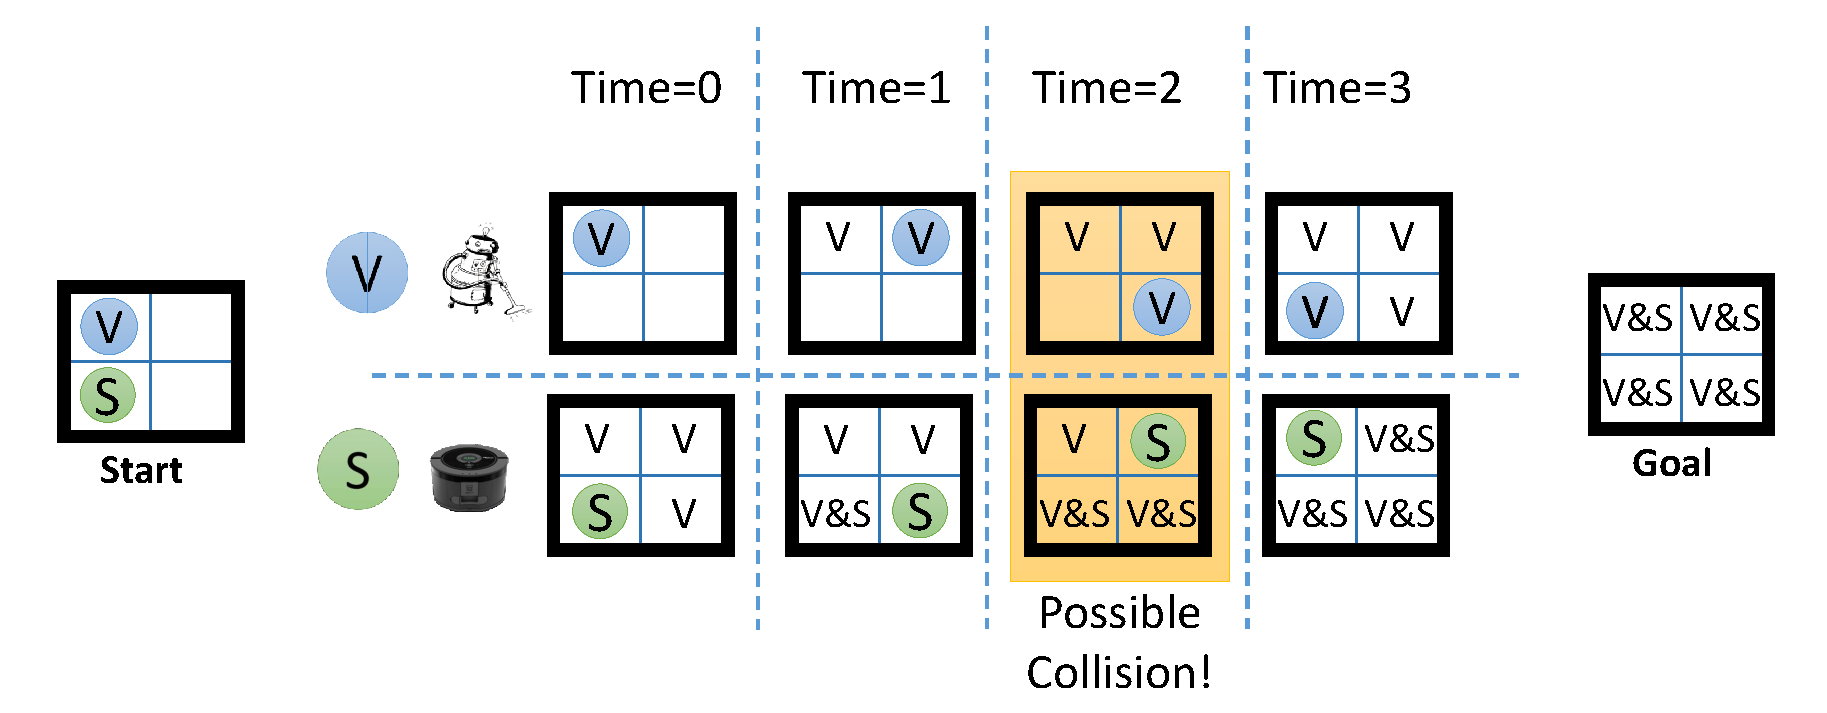
\includegraphics[width=0.8\columnwidth]{free-space_cropped.pdf}%
\vspace{-0.4cm}
\caption{{\small An example of generating provisional plans with the generalized free space assumption on a simplified version of our smart home example in Figure~\ref{fig:example} (using the same notations). 
Each provisional plan is displayed (robot V's plan in the upper line and robot S's plan in the lower line). The generalized free space assumption manifests in that (1) both plans ignore collisions and (2) robot S assumes all tiles are vacuumed. Indeed, 3 PIFs exists in this provisional plan: tiles (2,1) and (2,2) planned for scrubbing at time 0 and 1 will not be vacuumed in time (positive PIF) and a collision is expected at time 3 (negative PIF). Resolving them is discussed in later sections.}}
\label{fig:free-space}
\end{figure}


Fully coordinated planning and uncoordinated planning are two extremes of a spectrum of possible ways to generate provisional plans. We will also consider hybrid approaches, including:


{\bf 3. Planning under the generalized free-space assumption.} {\em Use uncoordinated planning but assume complete cooperation from other agents when planning for the individual agents.} 
An important limitation of using uncoordinated planning to generate provisional plans is that it is incomplete, in the sense that the provisional plans may not achieve some goals. This occurs for goals that cannot be achieved by any individual agent without assistance from other agents. 
Generating provisional plans by {\em planning under the generalized free-space assumption} is a middle ground between uncoordinated and coordinated planning, intended to resolve the incompleteness of uncoordinated planning without resorting to fully coordinated planning. Fast single-agent planners are used to generate the provisional plans, but these planners are modified to have some knowledge about what  other agents can achieve and assume their complete cooperation. This enables generating provisional plans even for goals that achieving them requires collaboration. 

We refer to the planning task performed by these modified single-agent planners as {\bf planning under the generalized free-space assumption}, as it was inspired by path finding algorithms that use the free-space assumption -- the assumption that unknown terrain does not have any obstacles -- as a heuristics~\cite{koenig2005fast}. In our smart home example, this generalized free-space assumption means that potential collisions between robots are ignored and that the floor scrubbing and floor mopping robots assume that the floor will be vacuumed by the vacuum cleaning robot before they start scrubbing/mopping the floor. Figure~\ref{fig:free-space} illustrates a simple example of planning under this assumption and the PIFs in the incumbent joint plan that is returned. 

Adapting single-agent planning algorithms to plan under the generalized free space assumption can be non-trivial, as it requires identifying what the other agents can achieve. This can be approximated by ignoring delete effects of the agents actions, as done in delete-relaxation heuristics~\cite{hoffmann2005ignoring,domshlak2015red,vstolba2014relaxation}, but that may result in assuming other agents can do anything. One way we will explore to control this is to only consider what other agents can achieve under a limited cost. Limiting this cost can also result in a more independent joint plan, requiring fewer refinements due to coordination. Also, implementing this assumption for domains that are not given in propositional logic is another challenge we will address.% cost of expected cooWe will explore  To limit the required coordination in provisional plans  generated  assumed at stage  between the agents at execution (or even planning) tim Moreover, the one may consider restricting this assumption to consider only what each agent can achieve under a limited cost, to limit the coordination between the agents at execution (or even planning) time.  

%In section~\ref{sec:} we discuss our approach for performing this type of planning in concrete MAP models. 
%The initial provisional plan of each agent is generated under the assumption of total cooperation from other agents. This assumption is {\bf a generalized form of the free-space assumption}, which is the assumption that unknown terrain does not have any obstacles.\footnote{The free-space assumption is often used as a heuristic by path-finding algorithms~\cite{koenig2005fast,koenig2004incremental}.} In our example, planning with this generalized free-space assumption means that potential collisions between robots are ignored and that 
%the floor scrubbing robot assumes that the floor will be vacuumed by the vacuum cleaning robot before it starts scrubbing the floor. %In section~\ref{sec:} we discuss our approach for performing this type of planning in concrete MAP models. 
%\subsubsection{Hybrid Approaches}
%Fully coordinated planning and uncoordinated planning are two extremes of a spectrum of possible ways to generate provisional plans. We will also consider the hybrid approaches, including:

{\bf 4. Coordinated planning for subsets of agents.} {\em Assign goals to agents as done in uncoordinated planning, partition the agents into groups and run a coordinated planner on each group independently.} This hybrid approach will be especially effective if the agents groups together are those agents that indeed require tight coordination while agents in different groups hardly require any coordination to achieve their goals. 
The challenge is to develop smart algorithms for grouping agents intelligently. We implemented such an approach in prior work on the development of the MA-CBS algorithm for solving MAPF problems~\cite{sharon2015conflict-based}. In MA-CBS, we detect conflicts (agents wanted to occupy the same location at the same time) between agents during planning, and agents that conflict frequently are grouped together and replanned together using coordinated planning. 

% and preliminary work on MA-STRIPS showed promise. 

{\bf 5. Coordinated planning of a relaxed MAP problem.} {\em Solve a relaxed version of the MAP problem using fully coordinated planning and then let the individual agents generate their provisional plans based on the joint plan generated for the relaxed problem.} Examples of possible MAP relaxations include by ignoring actions that do not directly affect other agents or ignoring delete effects of actions~\cite{hoffmann2005ignoring,domshlak2015red,vstolba2014relaxation}. We applied this approach successfully in our Greedy Privacy Preserving Planner (GPPP) for MA-STRIPS problems with privacy constraints~\cite{maliah2014privacyPreserving,maliah2015privacy}. 


Beyond developing all these approaches for generating provisional plans, an important contribution of the proposed research is in performing a thorough experimental comparison of these approaches over a range of domains. We do not expect any of the proposed approaches to dominate the others and thus a thorough experimental comparison can give insights as to how to customize the suitable approach for a given MAP problem. In addition, we will develop methods for generating provisional plans that integrate the above approaches, such as performing coordinated planning for subsets of agents on a relaxed MAP problem. 



\subsection{Analyzing and Refining the Provisional Plans}
\label{sec:analyzing}
The next stage in IOP is to continuously refine the generated provisional plans by searching for PIFs and resolving them. Following the classification of von Martial~\cite{martial1992coordinating}, we distinguish between two types of PIFs: negative and positive. A negative PIF arises if the execution of one provisional plan prevents the execution of another, e.g.,  if two robots plan to occupy the same location at the same time, or if one agent consumes a resource that another agent had planned to use in the future. Negative PIFs can be viewed as a generalization of the notion of ``mutexes'' used for single-agent planning~\cite{blum1997fast,smith1999temporal,bonet2000planning}, where plans have negative PIFs if their constituent actions are mutexes.  A positive PIF occurs when the success of the provisional plan of one agent depends on actions not included in the provisional plans of the other agents. 
%If the provisional plans were generated by planning under the generalized free-space assumption, then searching for PIFs is, in a sense, checking the validity of this assumption. %e generalized free-space assumption adopted at the time that these plans were generated. 

In MAP models that are based on propositional logic like MA-STRIPS~\cite{brafman2013complexity}, we formally define PIF by the tuple $\langle A,T,D\rangle$, where $A$ is the involved agents and $T$ is the type of PIF -- positive (denoted by P) or negative (denoted by N). For positive PIFs, $D$ is the fact that is needed by the provisional plans of the agents in $A$ but is not achieved by any agent. For negative PIFs, $D$ is the pair of actions that conflict. For example, the positive PIFs in Figure~\ref{fig:free-space} are  
$\langle [S], P, \vac{0}{(2,1)} \rangle$ and $\langle [S], P, \vac{1}{(2,2)} \rangle$, 
and the negative PIF is $\langle [V,S], N, \{ \move{V}{3}{(2,2)}, \move{S}{3}{(2,1)} \} \rangle$, where the predicate \vac{T}{F} means that floor tile $F$ is vacuumed at time $T$ and the predicate \move{R}{T}{F} means that robot $R$ moved to floor tile $F$ at time $T$. 

%The provisional plans in Figure~\ref{fig:free-space} have two positive PIF: $\langle [S], P, \vac{0}{(2,1)} \rangle$ and $\langle [S], P, \vac{1}{(2,2)} \rangle$ and one negative PIF: $\langle [V,S], N, \{ \move{V}{3}{(2,2)}, \move{S}{3}{(2,1)} \} \rangle$. The positive PIFs are for where robot S assumes that a floor tile will be vacuumed but the provisional plan of the robot V does not include vacuuming that tile on time. The negative PIF is for the collision that will occur at time 3 according to the current provisional plans. 

%In our example, a positive PIF exists if the floor scrubbing agent assumes that a given floor tile will be vacuumed, but the provisional plan of the vacuum cleaning robot does not include vacuuming that tile on time. 



%If the provisional plans were generated by planning under the generalized free-space assumption, then searching for PIFs is, in a sense, checking the validity of this assumption. %e generalized free-space assumption adopted at the time that these plans were generated. 
Searching for PIFs in a set of provisional plans is, in a sense, checking the validity of the assumptions (e.g., the generalized free-space assumption) adopted at the time that these plans were generated. 
The methods we will develop for identifying PIFs and the complexity of these methods will vary, depending on the type of PIF (negative or positive) and the MAP formalism used. For instance, identifying PIFs in a temporal planning setting is trivial: every action in the provisional plans is associated with a specific time, and PIFs can be detected by simulating the execution of the provisional plans.  For MAP models that are not temporal, identifying PIFs is more challenging, requiring, methods for identifying causal-link threats and open preconditions~\cite{cox2009efficient}. Clearly, an open precondition or an unresolvable causal-link threat pose a PIF. However, additional PIFs may be detected if we have some knowledge about the duration of performing each action and the time when agents plan to perform them. 


\subsubsection{Methods for Resolving PIFs}
\label{sec:methodsForResolving}
We will study two approaches for PIF resolution:  ``join and replan'' and ``constrain and replan''. 
The ``join and replan'' method considers the interacting agents as a single agent and replans for them as a whole using a baseline MAP solver. By construction, the originating PIF is resolved, as the generated plan is free of any PIFs between these agents. The complexity of the ``join and replan'' method depends on the MAP planner used, and can be exponential in the number of joined agents. 
The ``constrain and replan'' method attempts to avoid this exponential complexity by replanning only for one of the agents involved and constraining this agent's new plan to avoid the PIF. For a negative PIF, this constraint means avoiding the actions that caused it. For a positive PIF, it  means adding a subgoal of performing the task assumed by another agent's plan. 
Coordinating agents by adding incrementally adding constraints has been explored by Ephrati and Rosenschein~\cite{ephrati1993multi} but their focus was on self-interested agents aiming to avoid sharing their private goals and preferences. %that are self-interested, and adding constraints incrementally was done to avoid sharing private goals and preferences of the individual agents. 


% Many decisions to make
%The proposed PIF resolution mechanism chooses how to resolve a given PIF -- whether to ``join and replan'' or to ``constrain and replan''. 
%If the ``constrain and replan'' option is chosen, then the PIF resolution mechanism needs to choose which agent will replan with a newly added constraint (either to avoid an action or to perform a subgoal). More generally, the PIF resolution mechanism needs to pick which PIF resolution method to use. 

\begin{figure}%
\centering
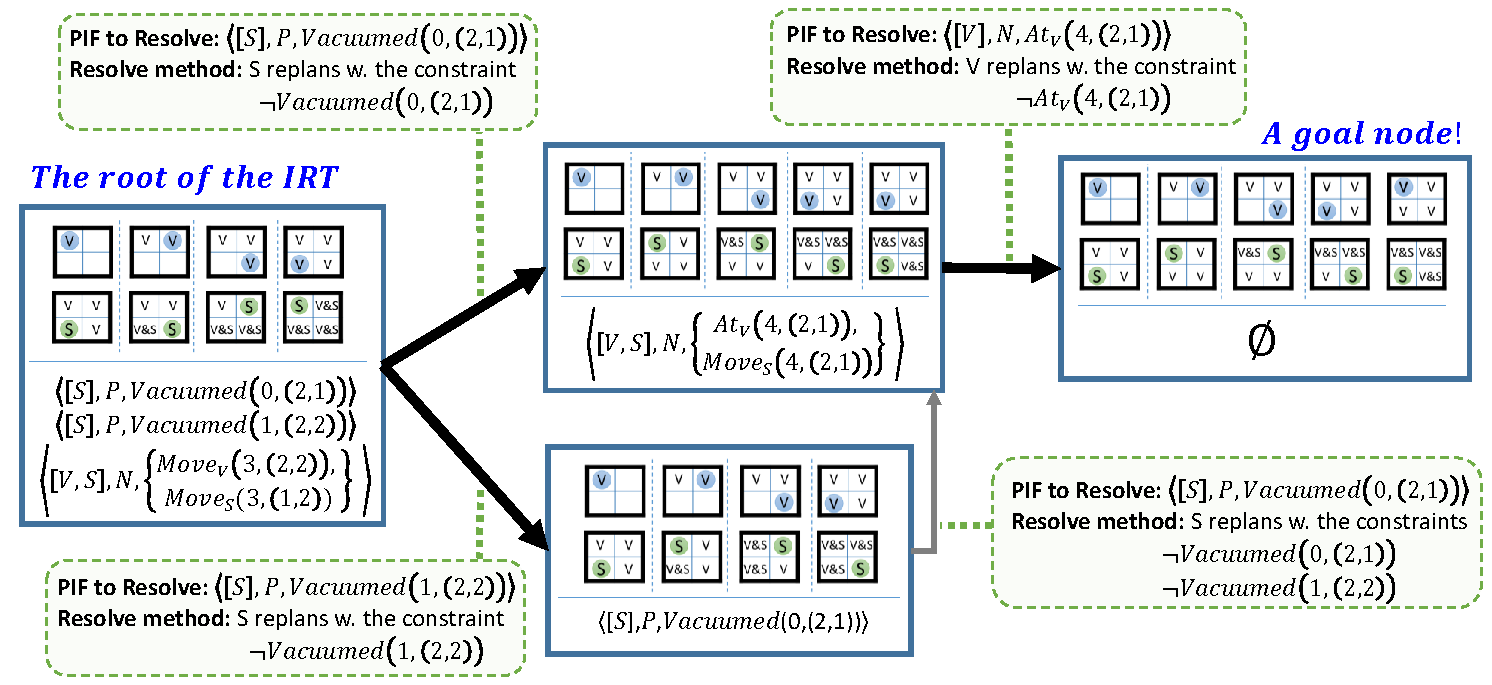
\includegraphics[width=0.8\columnwidth]{IRT-example_cropped}%
\vspace{-0.4cm}
\caption{{\small An IRT for solving the problem in Figure~\ref{fig:free-space}. Rectangles represent IRT nodes: the upper part of the rectangle shows the provisional plans, the lower part shows the PIFs, and we do not show the constraints to simplify the presentation. The IRT root node consists of the provisional plans generated using the generalized free-space assumption as shown in Figure~\ref{fig:free-space}. Every branch corresponds to choosing a PIF and resolving it. The chosen PIF and resolution method is given in the rounded rectangles. Any tree search algorithm can traverse this tree, and more branches can be generated. The goal node is an IRT node representing a joint plan without any PIF, and our example IRT has two possible paths to it.}}
\label{fig:irt-example}%
\end{figure}

A given PIF can be resolved by either of these  PIF resolution methods, resulting in different provisional plans and runtime. More generally, the entire MAP problem is viewed as a decision-making problem of choosing the PIFs to resolve and choosing how to resolve them. We propose to formalize this decision-making problem as a tree search problem. A node in this tree is a tuple consisting of (1) a set of provisional plans, (2) a set of PIFs identified for these plans, and (3) a set of constraints, previously imposed on the agents to resolve PIFs. The children of a node in this tree are all the ways to resolve one of the PIFs in that node. 
We call this tree the {\bf interaction resolution tree (IRT)} and propose to solve MAP by applying heuristic search algorithms on the IRT, searching for a node with provisional plans that can be executed. Figure~\ref{fig:irt-example} shows an example of an IRT for solving the MAP problem in Figure~\ref{fig:free-space}. 

%Resolving PIFs by searching the IRT generalizes our conflict-based search (CBS) algorithms (and its variants) in which solutions for MAPF are found by searching a tree of possible constraints to impose on the individual agents~\cite{sharon2015conflict-based,boyarski2015don,boyarski2015icbs}. In IOP, we go well beyond CBS in that CBS was designed for MAPF and not MAP in general, and thus CBS does not support positive PIFs, assumes predefined allocation of goals to agents, and do not consider deferring interaction resolution to execution (see Section~\ref{sec:resolving}). 

Resolving PIFs by searching the IRT generalizes our conflict-based search (CBS) algorithms (and its variants) in which solutions for MAPF are found by searching a tree of possible constraints to impose on the individual agents~\cite{sharon2015conflict-based,boyarski2015don,boyarski2015icbs}. Straightforward application of CBS to general MAP is not possible, since CBS was designed for MAPF and thus 
it ignores positive PIFs, assumes a given allocation of goals to agents, and do not consider deferring interaction resolution to execution (see Section~\ref{sec:resolving}). 

%In this research, we go well beyond CBS in that CBS was designed for MAPF and not MAP in general, and thus CBS does ignores positive PIFs, assumes predefined allocation of goals to agents, and do not consider deferring interaction resolution to execution (see Section~\ref{sec:resolving}). 
 


%This approach -- searching the IRT with a BFS -- to find a cost-optimal plan was applied by us in prior work in the development of a family of successful-optimal MAPF solvers~\cite{sharon2015conflict-based,boyarski2015don,boyarski2015icbs}. We expect to develop similarly successful algorithms using this approach for finding optimal joint plans in general-purpose MAP problems. 




%This can be viewed as a combination of state-space and plan-space planning, where generating the provisional plans can be done by a state-space planner but searching the IRT is in fact a search in the space of joint plans. Moreover, most plan-space planning algorithms do not provide any guarantees about the cost of the resulting joint plan, while searching the IRT allows doing so, as described next. 
% TODO: Consider putting this back in
%In an essence, MAP with IOP is a search in the IOP tree, where the goal is to find a node with provisional plans that will result in a sufficiently low execution cost.

\subsubsection{Finding a Cost-Optimal Joint Plan by Resolving Potential Interaction Failures}% Handling}

There are many possible ways to generate and search the IRT. For example, the IRT shown in Figure~\ref{fig:irt-example} has two paths leading to a PIF-free joint plan, and that IRT is but one of many possible IRTs one could generate to solve the same problem. Therefore, a major theme of the proposed research is in the development of smart algorithms for searching the IRT cost-effectively. % Theoretical analysis
Using a systematic heuristic search algorithm to search the IRT provides {\bf flexible control over the cost of the joint plan it produces}.\footnote{The cost of a joint plan can be defined in multiple ways, and we will focus on joint plan cost functions that aggregate the costs of the joint plan's constituent individual plans (e.g., summing their costs).} 
For a given IRT node $n$, let $cost(n)$ denote the cost of the incumbent joint plan in $n$, and let $cost^*(n)$ denote the cost of the best joint plan reachable by continuously refining the incumbent joint plan in $n$.
By analyzing the relationship between $cost(n)$ and $cost^*(n)$ and using suitable tree-search algorithms, it is possible to find provably optimal solutions by searching the IRT. 


%Thus, tuning IOP to find optimal joint plans can be done as follows.
\begin{corollary}[Cost-Optimal Joint Plan]
If for every IRT node $n$ it holds that $cost(n)\leq cost^*(n)$ then searching the IRT in a best-first search (BFS) where nodes are ordered according to the cost of their incumbent joint plan 
will return a joint plan with optimal cost. 
\label{cor:optimal}
\end{corollary}
The BFS described in Corollary~\ref{cor:optimal} is optimal because it is a special case of the BF$^*$ algorithm~\cite{dechter1985generalized}, which is a BFS that expands nodes according to a $f(n)$ function that is required to be admissible (lower bound). BF$^*$ is a general version of the well-known the \astar\ algorithm~\cite{dechter1985generalized,hart1968formal}. 
The condition $cost(n)\leq cost^*(n)$ holds in cases where provisional plans are generated by planning under the generalized free-space assumption. 
This is because the provisional plans of any IRT node $n'$ in a subtree rooted at $n$ must adhere to at least the set of constraints as in $n$, and thus $cost(n)\leq cost(n')$. $cost(n)\leq cost^*(n)$ also holds if provisional plans are generated using the coordinated planning of a relaxed MAP problem approach for certain types of MAP relaxations. We will study the exact conditions when $cost(n)\leq cost^*(n)$, facilitating the development of efficient cost-optimal MAP planners. 
% TODO: Talk about lower bound
This approach -- searching the IRT with a BFS -- to find a cost-optimal plan was applied by us in prior work on MAPF, resulting in the development of a family of successful-optimal MAPF solvers~\cite{sharon2015conflict-based,boyarski2015don,boyarski2015icbs}. We expect to develop similarly successful algorithms using this approach for finding optimal joint plans in general-purpose MAP problems. 



\subsubsection{Trading Plan Optimality for Efficiency}
\label{sec:tradingPlan1}
Finding an optimal joint plan is often not needed, and quickly obtaining a suboptimal joint plan is preferred. % over waiting a long time to find optimal solutions. 
Moreover, finding optimal joint plans can be intractable in practice. Thus, for practical purposes optimality must often be relaxed. We propose to develop and analyze several complementary approaches for introducing suboptimality and study how these approaches can be combined to achieve the best performance. 

% We could use bounded suboptimal search algorithms but it requires some modifications
{\bf Suboptimal search of the IRT.} 
This approach introduces suboptimality by searching the IRT with a suboptimal search algorithm. Most bounded-suboptimal search algorithms~\cite{pohl1973avoidance,pearl1982studies,thayer2011bounded} rely on an evaluation function in the form of $f_w(n)=g(n)+w\cdot h(n)$, where $w$ is the desired amount of suboptimality, $h(n)$ is a lower bound on the lowest cost of reaching a goal from $n$, and $g(n)$ is the cost spent to reach $n$ from the start state. Adapting such algorithms to search the IRT for suboptimal solutions is non-trivial, as there is no obvious lower bounding heuristic function ($h(n)$), since the notion of ``path cost'' between nodes is meaningless in the IRT, as cost is associated with nodes (the cost of the incumbent joint plan) and not edges. 

% This can be solved with EES, but we need distance and inadmissible estimates 
To resolve this challenge, we will explore an approach based on Explicit Estimation Search (EES)~\cite{thayer2011bounded}, a state-of-the-art bounded suboptimal search algorithm. To choose which nodes to expand, EES uses a combination of evaluation functions: $f(\cdot)$, $\hat{f}(\cdot)$, and $d(\cdot)$. $f(n)$ and $\hat{f}(n)$ are both estimates of the cost of the optimal path to the goal that passes through $n$. $f(n)$ is an admissible (lower bound) estimate of the optimal cost, while $\hat{f}(n)$ is inadmissible, and thus potentially more accurate than the $f(n)$. $d(n)$ is an estimate of the number of operators needed to reach the goal, which serves as a rough estimate of the search effort required to find  beneath node $n$ a goal with the desired suboptimality. EES intelligently combines $f(n)$, $\hat{f}(n)$, and $d(n)$ to effectively find a solution whose cost is at most $w$ times the optimal solution, where $w$ is a parameter chosen by the user.


Applying EES to find joint plans in the IOP tree requires developing effective $f(n)$, $\hat{f}(n)$, and $d(n)$ suitable for searching the IOP tree. If $cost(n)$ is an admissible lower bound, it can be used instead of $f(n)$. If not, we will investigate other ways to generate lower bounds on $cost^*(n)$, e.g., by using cost-partitioning techniques on the provisional plans such as those used for adding multiple abstraction heuristics~\cite{katz2010optimal}. We have begun to explore ways for analyzing the PIFs in the provisional plans to estimate the distance to a goal ($d(n)$), with preliminary results suggesting that this is a promising approach~\cite{barer2014suboptimal-socs}. We will also explore using machine learning methods to learn from past planning sessions the relation between various problem properties and the most suitable PIF resolution mechanism, thus providing additional guidance for searching the IRT. 

%Distance estimates based on  analyzing the negative interaction failures in the provisional plans were shown to be highly effective in our preliminary work on the MAPF problem~\cite{barer2014suboptimal-socs,barer2014suboptimal-ecai}. Generalizing these ideas to general MAP, where positive interaction failures also occur is part of this proposal. 


{\bf Suboptimal baseline planner.} 
A different way to add suboptimality is by allowing the baseline planner to find provisional plans that are suboptimal. Importantly, the ``amount'' of suboptimality of the resulting joint plan is derived from the ``amount'' of suboptimality of the provisional plans. Thus, for example, if the baseline planner is tuned to find solutions that are at most $1.1$ times the optimal plan, then the overall joint plan is also at most $1.1$ times of the optimal joint plan. More generally, if the cost of a joint plan is the sums of costs of its constituent plans and the baseline planner returns for each agent $a_i$ a plan of cost $cost_i$ with a bound $w_i$ on the suboptimality of this plan, then the suboptimality of the joint plan is $\frac{\sum_{i=1}^k cost_i}{\sum_{i=1}^k \frac{cost_i}{w_i}}$.  

{\bf Inadmissible estimates of cost.}
The above approaches for adding suboptimality rely on having a lower bound on $cost^*(n)$. Obtaining such a lower bound may be difficult in some domains. An alternative approach we will study and develop is to {\bf guide the BFS of the IRT with an inadmissible estimate of $cost^*(n)$}, i.e., estimates that may not be a lower bound. Such heuristic estimates can be obtained, for example, by applying Machine Learning methods to learn an estimator $\widehat{cost}(n)$ of $cost^*(n)$ from MAP problems solved in the past. 
In prior work, we developed the theory for obtaining probabilistic guarantees on solution quality from such case, namely, guaranteeing that the returned solution is approximately optimal with high probability~\cite{stern2011probably,stern2012search}. 
%While having strict bounds on the joint plan cost is not possible when using inadmissible cost estimators, we have developed in prior work the theory to obtain probabilistic guarantees on solution quality from such estimators~\cite{stern2011probably,stern2012search}, namely, guaranteeing that the returned solution is approximately optimal with high probability. 


In our preliminary work on solving the restricted MAPF problem suboptimally, we found that using a combination of some of the approaches above enabled scaling to more than a hundred agents while allowing only 1\% suboptimality~\cite{barer2014suboptimal-socs}. Generalizing to general-purpose MAP is, however, much more challenging. 


\subsection{Resolving Potential Interaction Failures During Execution Instead of Planning}
%\subsection{Deferring Resolution of Potential Interaction Failures to Execution}
\label{sec:resolving}
%\item {\bf To develop a method for identifying potential interactions that are safe to ignore during planning

% Idea: defer resolving failures to runtime
Agents often have capabilities to resolve problems that arise during the execution of their plans. For example, many robots have collision avoidance and other control procedures. 
Thus, some PIFs identified in an incumbent joint plan can be left unresolved during planning, with the expectation that agents will be able to detect and resolve them during execution. In our example, the  scrubbing robot may be able to detect that the floor has not been vacuumed yet and invest more time to clean it more thoroughly. %in cleaning the floor to achieve the same level of cleanliness. 
Some PIFs can be easily resolved during execution but for others it may be very costly. It may even be that a PIF cannot be resolved during execution, thereby causing the entire mission to fail. A key question is which PIFs can be ignored when planning. 
% TODO: Add an example

%results in a system failure (if a failure is not hancan only be detected during execution at a stage where avoiding it is impossible.


% Approach: SharedPlans gives us the separation of "planing" and knowing that "can bring about"

%The approach we will explore for answering this question is based on the claim that a PIF can be ignored if it is known that the involved agents will be able to achieve their goals, i.e., the PIF will be resolved during execution. 
The approach we will explore for answering this question is based on the claim that a PIF can be ignored if it can be resolved during execution, i.e., if the agents involved will be able to achieve their goals regardless of the PIF (replanning during execution if needed). This claim can be stated in terms of a  special case of the SharedPlans ``can bring about group'' predicate ($cbag$), which states that a group of agents is able to achieve some task~\cite{grosz1996collaborative}. In the context of resolving PIFs, the task referred to by the $cbag$ predicate is the agents achieving their goals, given the incumbent joint plan and its PIFs.  
For example, consider two agents that have been tasked to reach two different locations and have access to two cars. Even if their provisional plans intend to use the same car, there is no need to resolve this negative PIF as long as the agents know they can resolve it during execution, i.e., they know that they each will have a car at the requisite time. 



\subsubsection{Computing ``Can Bring About Group''}
\label{sec:computing}
% How to implement cbag: 1) Predifined recipes
Computing $cbag$ efficiently for a set of provisional plans presents both theoretical and algorithmic challenges, requiring the prediction of what the agents can achieve without generating a plan to achieve it. We will investigate the following approaches to computing $cbag$. 

{\bf 1. Computing $cbag$ by relying on pre-defined recipes for PIF identification and resolution.} 
In some domains, the agents are capable of identifying PIF during execution and apply predefined recipes for handling them. 
For example, robots may have predefined {\em behaviors} (corresponding to recipes in SharedPlans terminology) for detecting and avoiding collision with other agent and for swapping locations with an adjacent robot. Such behaviors are sufficient to enable all robots to reach their goal locations under very general settings~\cite{wang2009tractable,snape2011hybrid,de2013push}. Importantly, there is no need during planning time to plan exactly how every specific potential collision will be handled, as we know that every collision will be detected and avoided. This allows much faster planning as PIFs related to collisions can be ignored during planning, and computational resources can be allocated to resolve other PIFs. For example, searching the IRT in Figure~\ref{fig:irt-example} could halt earlier if the negative PIF: $\langle [V,S], N, \{ \at{V}{4}{(2,1)}, \move{S}{4}{(2,1)} \} \rangle$ is ignored.

%In some domains, $cbag$ can be computed from domain and agent models or characteristics. For example, robots may have predefined behaviors (corresponding to recipes in SharedPlans terminology) for how to avoid a collision if one is detected and for swapping locations with an adjacent robot. Such behaviors are sufficient to enable all robots to reach their goal locations under very general settings~\cite{wang2009tractable,snape2011hybrid,luna2011push,de2013push}. Importantly, generating the exact plan detailing how these conflicts are avoided is not needed, and will be done during execution. This allows much faster planning Thus, PIFs related to collisions can be ignored during planning, and computational resources can be allocated to resolve other PIFs. 

% How to implement cbag: 2) Domain abstraction
%A more general way to compute $cbag$ is to use abstractions of the original domain.  Thus, to check whether a group of agents can resolve their interaction failure at runtime, an abstract plan is generated to resolve this failure at plan time. The type of abstraction needs to be carefully chosen, such that abstract plans could be grounded to concrete ones at execution. 

{\bf 2. Estimating $cbag$ by resolving PIFs in a relaxed MAP problem.} 
Estimating whether the agents will be able to resolve a PIF can be done by {\bf trying to resolve it in a relaxed version of the original MAP problem}.  The high-level idea we propose is to estimate $cbag$ for a PIF in an incumbent  joint plan by checking if that PIF can be resolved in the relaxed MAP problem. Possible ways to relax a given MAP problem which we will investigate include ignoring delete effects of agents' actions~\cite{hoffmann2005ignoring,domshlak2015red,vstolba2014relaxation} and abstracting some of the state variables~\cite{edelkamp2001planning,korf2002disjoint,felner2004additive,helmert2014merge,maliah2015privacy}. An example of the latter type of relaxation is to ignore limitations on robots' motion that are due to kinematic constraints.
The effectiveness of estimating $cbag$ by considering a relaxed MAP problem depends on two properties of the used relaxation: {\em efficiency} -- planning in the relaxed MAP problem should be much faster than in the original domain, and what we refer to as {\em groundability} -- finding a plan in the abstract domain should suggest that it is likely for such a plan to exists in the original domain. We will investigate effective problem relaxations that balance these desirable properties, taking into consideration the specific MAP problem being solved. We successfully applied this approach in our preliminary work on GPPP for privacy-preserving MAP~\cite{maliah2014privacyPreserving,maliah2015privacy}. 








%Abstractions and problem relaxations are commonly used to generate heuristics for search algorithms~\cite{edelkamp2001planning,korf2002disjoint,felner2004additive}. 

%Thus, the type of abstraction needs to be carefully chosen. Choosing the appropriate form of domain abstraction and identifying how likely it is that a PIF resolved in the abstract problem would also be resolved in the real problem are some of the challenges we plan to address.



%The high-level idea we propose to explore is to is that resolving a PIF in this relaxed problem can be done very fast, and if a PIF can be resolved in a relaxed version of the MAP problem then it is likely to be resolvable in the original problem. For example, to check if robots can avoid a future collision, one can plan how these robots can avoid that collision in a simpler, gridworld abstraction of the real world, and leave to execution the much more costly high-dimensional motion planning task of avoiding this collision that considers additional kinematic constraints. The type of abstraction needs to be carefully chosen, such that abstract PIF resolving plans are likely to be groundable to concrete ones at execution. Choosing the appropriate form of abstraction and identifying how likely it is that a PIF resolved in the abstract problem would also be resolved in the real problem, are some of the challenges we plan to address.


%A simplified version of our example is, for instance, to plan for the robots without considering motion planning considerations, thus planning under the assumption that robots can move to any location they choose.  constraints. 




%A different and more general way to estimate $cbag$ is to use a relaxed verconsidering an abstract of or other some other relaxed version of the MAP problem. The high-level idea is that resolving a PIF in this relaxed problem can be done very fast, and if a PIF can be resolved in a relaxed version of the MAP problem then it is likely to be resolvable in the original problem. For example, to check if robots can avoid a future collision, one can plan how these robots can avoid that collision in a simpler, gridworld abstraction of the real world, and leave to execution the much more costly high-dimensional motion planning task of avoiding this collision that considers additional kinematic constraints. The type of abstraction needs to be carefully chosen, such that abstract PIF resolving plans are likely to be groundable to concrete ones at execution. Choosing the appropriate form of abstraction and identifying how likely it is that a PIF resolved in the abstract problem would also be resolved in the real problem, are some of the challenges we plan to address.


%an abstract version relaxed version of original problem. For example, by lowerign use abstractions of the original domain.  Thus, to check whether a group of agents can resolve their interaction failure at runtime, an abstract plan is generated to resolve this failure at plan time. The type of abstraction needs to be carefully chosen, such that abstract plans could be grounded to concrete ones at execution. 

%Preliminary work on defining the required collaboration in a STRIPS formalism~\cite{zhang2014formal}


%In the proposed research we intend to develop the above approaches for identifying when interaction failures can be ignored while keeping the agents' mission achievable.

\subsubsection{Trading Plan Reliability and Cost for Efficiency}
\label{sec:tradingPlan2}
Ignoring PIFs in planning and resolving them during execution may introduce suboptimality. For example, the paths resulting from using an ad-hoc collision avoidance behavior may be less efficient than planning upfront non-colliding paths for the robots. 
For an IRT node $n$, we denote by $xcost(n)$ the cost of executing its provisional plans as is, without resolving its PIFs during planning. $xcost(n)$ can be viewed as a quantitative extension of the $cbag$ predicate, answering not just whether the group can resolve a PIF but also what would be the cost of doing so. The suboptimality resulting from executing the provisional plans in $n$ is given by $xcost(n)-cost^*(n)$ and denoted as $\Delta_x(n)$. 

%The difference between $cost^*(n)$ and $xcost(n)$, denoted $\Delta_x(n)$, is the added execution cost resulting from ignoring the PIFs in $n$. In other words, the suboptimality resulting from executing the provisional plans in $n$ is $\Delta_x(n)$. 


Exactly computing $\Delta_x(n)$ is not possible, since $cost^*(n)$ is usually not known before the MAP problem is solved and $xcost(n)$ is not likely to be known prior to execution. To bound the suboptimality of a returned joint plan, we will explore methods for bounding $\Delta_x(n)$. 
An approach we intend to take is to generate a lower bound heuristics, $h(n)\leq cost(n)$, and an upper bound heuristic $h_x(n)\geq xcost(n)$, and then bounding $\Delta_x(n)$ by $h_x(n)-h(n)$. 
Above we discussed ways to develop a lower bounding $h(n)$ and shown that in some cases $cost(n)$ itself can be used as $h(n)$. To generate an upper bounding heuristic $h_x(n)$, we will investigate generating $h_x(n)$ using similar approaches to those described for estimating $cbag$; namely, $xcost(n)$ can be estimated by analyzing existing recipes for resolving PIFs (e.g., collision avoidance protocols), or by considering a relaxed version of the original MAP problem where estimating the execution cost can be done faster. 

%Another way to achieve Deferring handling of PIFs to execution time opens the possibility of rea 


\subsection{Methodology and Experimental Evaluation}
\label{sec:methodology}
The main MAP model we will use for evaluating IOP and its different components is MA-STRIPS~\cite{brafman2013complexity}. MA-STRIPS can be viewed as the simplest extension of the classical STRIPS planning formalism. An MA-STRIPS problem is defined exactly like a STRIPS problem, with the only difference being that in MA-STRIPS each agent has a set of actions it can perform. MA-STRIPS is a relatively recent MAP model that has gained recent popularity~\cite{nissim2014distributed,vstolba2014relaxation,brafman2013complexity,zhang2014formal,komenda2013domain,torreno2014fmap,maliah2014privacyPreserving,maliah2015privacy,torreno2015global,jakubuv2015multiagent}.  In fact, there is an international competition for comparing MA-STRIPS planners~\cite{vstolba2015competition}. 
The competition organizers graciously made the code for all competing planning algorithms as well as all the problems used in this competition available to the community. This will allow us to compare the IOP-based MA-STRIPS planning algorithms we will develop against the state-of-the-art MA-STRIPS planners on a standard set of benchmark domains. MA-STRIPS serves as a ``lab'' setting, and we intend to evaluate IOP on a range of problems and settings listed below.

{\bf 1. Search-Based Planning for Teams of Robots.}
% We will evaluate on search-based multi-robot planning
%Planning for a team of robots provides one of the motivations for this research. Implementing IOP on real robots is beyond the scope of this research and requires additional expertise and funds. As a step towards realizing IOP on robot teams, we will implement IOP on top of the Search-Based Planning Library (SBPL)~\cite{likhachev2010sbpl}, a successful framework for applying search-based planning algorithms for robots.
Implementing IOP on real robots is beyond the scope of this research and requires additional expertise and funds. Bust, as a step towards realizing IOP on robot teams we will implement IOP on top of the Search-Based Planning Library (SBPL)~\cite{likhachev2010sbpl}, a successful framework for applying search-based planning algorithms for robots. 
SBPL is integrated with the Robotic Operating System (ROS), to allow relatively easy deployment to real robots and integration with standard ROS simulators. It was used in a range of robotic platforms such as a single robotic arm~\cite{stern2014potential,aine2015learning}, multiple robotic arms~\cite{cohen2014planning}, Willow Garage’s PR2~\cite{phillips2012graphs}, and an autonomous vehicle~\cite{likhachev2009planning}. 

We have started to develop a multi-robot extension of SBPL (MR-SBPL) and in a preliminary study compared planning with \astar\ to a simplified version of IOP. The particular domain was a MAPF variant: every robot had a goal location it needed to reach, and the state variables were $x$, $y$, and $\theta$, where $\theta$ is the orientation of the robot. On an experiment with 10 robots on randomly chosen start and goal locations that were 10 steps afar, we observed a speedup of a factor of 2 for IOP over \astar . In the proposed research, we will continue this study, extending MR-SBPL to richer domains with positive PIFs and non-static allocation of goals to agents. Note that we do not presume to develop real-life robotic applications in the proposed research as that would require dealing with various control issues (action failures, inaccurate sensors etc.). 

{\bf 2. Planning for Data Mules.} Data mules is a rising architecture for maintaining low-cost high latency networks, where mobile agents carry data between the network nodes~\cite{shah2003data}. %E.g., when  deploying a communication network is not feasible.
There are several planning tasks for data mules, including route planning~\cite{sugihara2011path} and handling network node failures~\cite{crowcroft2016using}. We will evaluate IOP against existing solutions for data mules problems. This will provide both practical benefit to real-life application as well as help cross fertilization with other communities.



{\bf 3. Decentralized POMDP.} We will implement IOP in more complex MAP models that directly address these issues during planning such as Dec-POMDP~\cite{bernstein2002complexity}, building on the MADP toolbox.  % of Dec-POMDP algorithms~\cite{MADPToolbox-0.3.1}. 



{\bf 4. Single agent search.} As noted above, we also intend to experiment with applying IOP to solve single agent problems. To this end we will experiment on standard domain-independent planning problems, and explore  using IOP with various domain decomposition methods~\cite{nissim2012tunneling,amir2003factored}. 





%\begin{figure}[t]
%\centering
%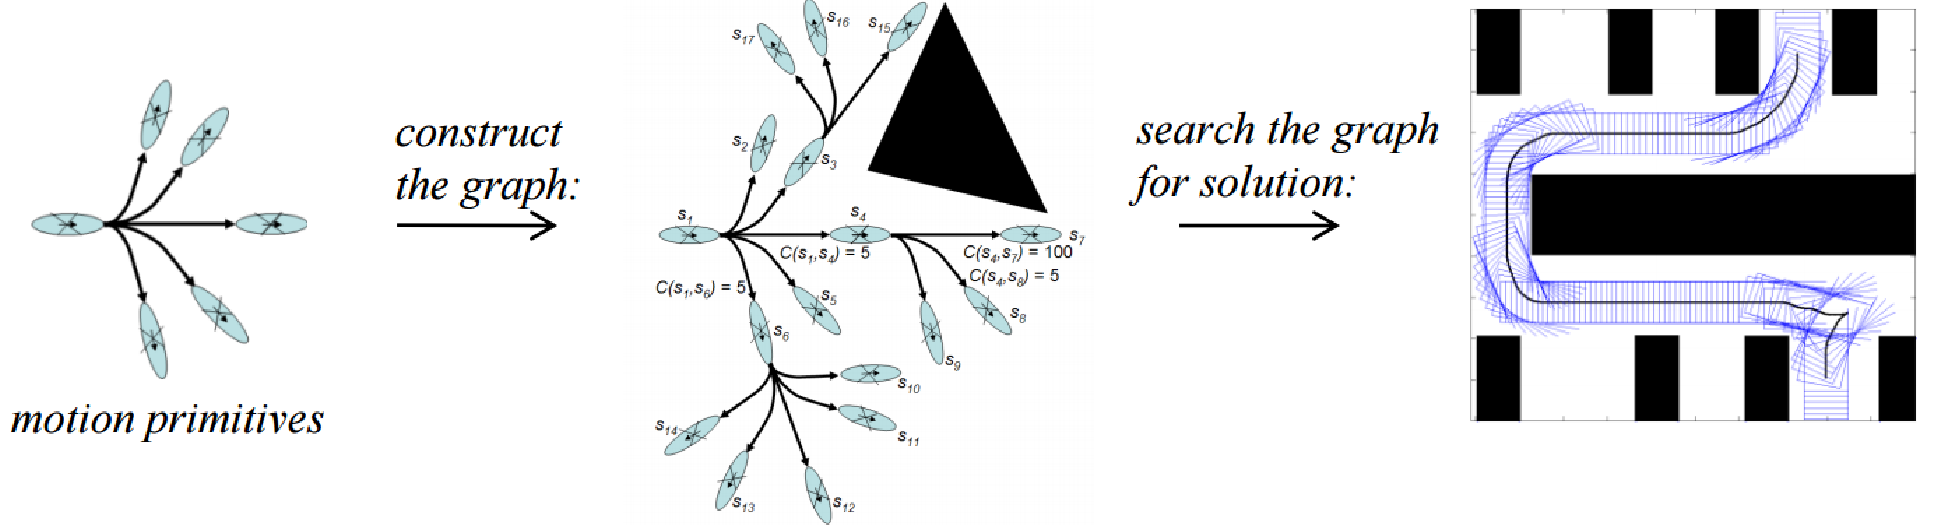
\includegraphics[width=0.8\columnwidth]{MotionPrimitives_cropped2} 
%\vspace{-0.4cm}
% \caption{An illustration of search-based planning with motion primitives (from slides by Maxim Likhachev)} \label{fig:motion-primitives}
%\end{figure}



\section{Available Resources}
Selected graduate students from our research group, which  currently consists 10 graduate students will participate in the proposed research. The facilities available at BGU for PI Stern's lab will be available for this research, including basic office facilities and a server for performing heavy duty computations. 







\pagebreak
\small
\bibliographystyle{plain}
%\bibliography{library-ast}
\bibliography{library}

\end{document}

